%!TEX root=../GaugeCNNTheory.tex


\section{شبکه‌های کانولوشنی مستقل از مختصات اقلیدسی}
\label{sec:instantiations_euclidean}

این بخش به بررسی کانولوشن‌های هموردا در فضاهای اقلیدسی (افاین) $M = \Euc_d$ می‌پردازد که بدون شک از بیشترین اهمیت عملی برخوردار هستند.
شبکه‌های کانولوشنی در فضاهای اقلیدسی برای تحلیل تصاویر صفحه‌ای و حجمی، سیگنال‌های صوتی، ویدئوها، رویدادهای فیزیکی در فضازمان مینکوفسکی (شبه-اقلیدسی) یا محیط‌های صفحه‌ای در یادگیری تقویتی به کار می‌روند.
معماری مدل کانولوشنی نمونه اولیه -- هم در فضاهای اقلیدسی و هم به طور کلی -- \CNN متعارف روی~$\Euc_d$ توسط \citet{LeCun1990CNNs} است.
موفقیت آن تا حد زیادی بر پایه هموردایی نسبت به انتقال است که به آن امکان تعمیم استنتاج آموخته‌شده بین مکان‌های فضایی مختلف را می‌دهد.
با انگیزه از این مشاهده، تلاش زیادی برای تعمیم ویژگی‌های هموردایی \CNN ها به گروه‌های تقارن \emph{سراسری} بزرگترِ~$\Euc_d$، به عنوان مثال به ایزومتری‌های اقلیدسی در شکل~\ref{fig:isometries_plane} یا تبدیلات افاین عمومی‌تر، صورت گرفته است.


جالب اینجاست که اکثر مدل‌های هموردای \emph{سراسری} در مقالات، هموردایی خود را با اعمال نوعی کرنل \lr{G}-راهبری‌پذیر به دست می‌آورند.
این بدان معناست که این مدل‌ها در واقع تحت تبدیلات پیمانه‌ای \emph{محلی} نیز هموردا هستند، علی‌رغم اینکه صراحتاً برای آن طراحی نشده‌اند.
دلیل این هموردایی پیمانه‌ای ناخواسته این است که هموردایی سراسری مدل‌ها معمولاً برای هر لایه به صورت جداگانه طراحی می‌شود و بنابراین به طور مستقل برای میدان دریافتی محلی هر نورون اعمال می‌گردد.
در اینجا ما \CNN های اقلیدسی هموردای سراسری را که در ردیف‌های (۱-۲۶) جدول~\ref{tab:network_instantiations} فهرست شده‌اند، از دیدگاه عمومی‌تر تقارن‌های پیمانه‌ای محلی توضیح می‌دهیم و بحث می‌کنیم که چگونه هموردایی سراسری آنها از هموردایی پیمانه‌ای محلی‌شان ناشی می‌شود.
قضیه~\ref{thm:isom_equiv_GM_conv} بدین ترتیب بیان می‌کند که یک کانولوشن $\GM$ روی $M = \Euc_d$ نسبت به $\IsomGM$ هموردا است.
با این حال، برای مورد خاص فضاهای اقلیدسی، می‌توان گزاره‌ای قوی‌تر از صرفاً هموردایی ایزومتری بیان کرد:
کانولوشن با یک کرنل \lr{G}-راهبری‌پذیر روی $\Euc_d$ به معنای هموردایی سراسری مدل تحت عمل گروه افاین $\Aff(G) := \Trans_d \rtimes G$ است، همانطور که در قضیه~\ref{thm:affine_equivariance_Euclidean_GM_conv} در ادامه اثبات شده است.
دلیل اصلی این نتیجه آن است که ژئودزیک‌ها و انتقال‌دهنده‌های لوی-چیویتا در فضاهای اقلیدسی نه تنها توسط ایزومتری‌ها حفظ می‌شوند، بلکه به طور کلی‌تر توسط هر تبدیل افاین نیز حفظ می‌گردند.

\begin{figure}
	\centering
	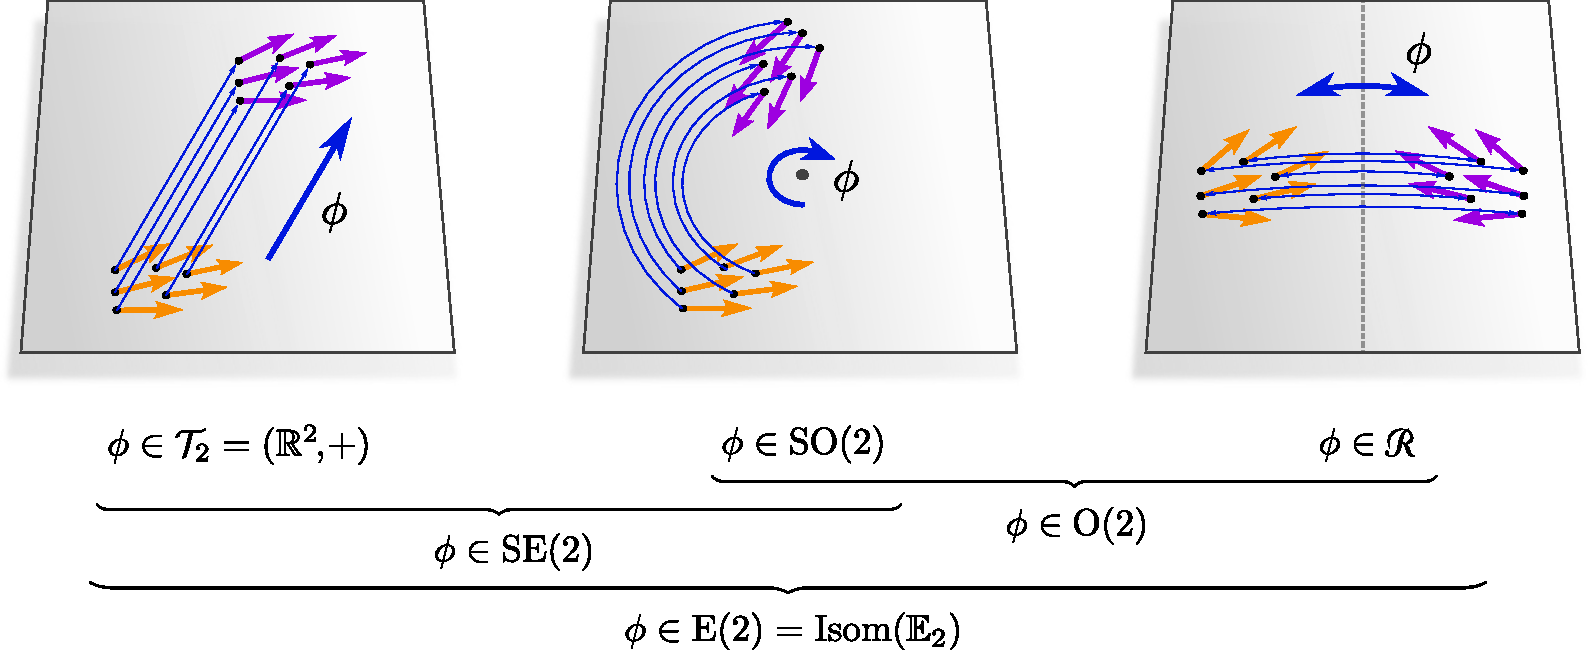
\includegraphics[width=1.\textwidth]{figures/isometry_plane.pdf}
	\vspace*{.1ex}
	\caption{\small
		نمایش گروه ایزومتری کامل $\Isom(\Euc_d) = \E{d}$ فضاهای اقلیدسی~$\Euc_d$ برای $d=2$.
		این گروه شامل زیرگروه‌های انتقال $\Trans_d \mkern-1mu=\! (\R^d,\mkern-2mu+)$، دوران $\SO{d}$ و بازتاب $\Flip$ است.
		دوران‌ها و بازتاب‌ها گروه متعامد ${\O{d} \!=\! \SO{d} \!\rtimes\! \Flip}$ را تشکیل می‌دهند، در حالی که انتقال‌ها و دوران‌ها گروه اقلیدسی خاص $\SE{d} = \Trans_d \rtimes \SO{d}$ را می‌سازند.
	}
	\label{fig:isometries_plane}
\end{figure}

کانولوشن‌ها در فضاهای اقلیدسی به طور کلاسیک \emph{در مختصات} $\R^d$ از $\Euc_d$ فرمول‌بندی می‌شوند.
مزیت این نوع فرمول‌بندی این است که $\R^d$ تمام ساختارهای ریاضی مورد نیاز برای تعاریف را فراهم می‌کند.
با این حال، $\R^d$ دارای ساختار اضافی است، به عنوان مثال یک ساختار فضای برداری (و در نتیجه یک مبدأ) یا ساختار کانونیک $\{e\}$ آن.
با طراحی کانولوشن‌ها به گونه‌ای که هموردا باشند، استنتاج (تا حدی) مستقل از این ساختار می‌شود:
به عنوان مثال، هموردایی نسبت به انتقال در کانولوشن‌ها، انتخاب خاص مبدأ را یکسان می‌سازد در حالی که هموردایی نسبت به $\E{d}$ (ایزومتری)، جهت و جهت‌گیری خاص ساختار $\{e\}$ را یکسان می‌کند.
برای روشن شدن اینکه کدام ساختار ریاضی واقعاً فرض و مورد نیاز است، ما یک دیدگاه جایگزین را توسعه می‌دهیم:
ما با ساختار خالص افاین و متریک فضای اقلیدسی~$\Euc_d$ شروع می‌کنیم.
اگر~یک کانولوشن $\GM$ روی $\Euc_d$ ساختار هندسی بیشتری را فرض کند، این ساختار متعاقباً با مشخص کردن اطلسی از چارت‌های (افاین) $x^A: \Euc_d \to \R^d$ که پیمانه‌ها و \lr{G}-ساختارها را القا می‌کنند، اضافه خواهد شد.

\pagebreak

\etocsettocdepth{3}
\etocsettocstyle{}{} % from now on only local tocs
\localtableofcontents


برای ارائه یک نمای کلی و مقدمه‌ای ساده، ما فرمول‌بندی کلاسیک کانولوشن‌های \lr{G}-راهبری‌پذیر (هموردای افاین) را در مختصات $\R^d$ در بخش~\ref{sec:steerable_cnns_in_coords} مرور می‌کنیم.
بخش‌های بعدی~\ref{sec:euclidean_geometry} و~\ref{sec:euclidean_affine_equiv} کانولوشن‌های هموردای افاین را در فضاهای اقلیدسی در یک چارچوب بدون مختصات و مستقل از مختصات تعریف می‌کنند.
به طور خاص، بخش~\ref{sec:euclidean_geometry} به بحث در مورد هندسه افاین فضاهای اقلیدسی می‌پردازد.
اطلس‌هایی از چارت‌ها با توابع گذار در یک گروه افاین $\Aff(G)$ (شکل~\ref{fig:affine_charts})، \lr{G}-ساختارهای ثابت تحت $\Aff(G)$ مورد نظر را القا می‌کنند (شکل~\ref{fig:G_structures_R2_main}).
بخش~\ref{sec:euclidean_affine_equiv} کانولوشن‌های $\GM$ را روی این \lr{G}-ساختارها بررسی کرده و هموردایی سراسری آنها نسبت به $\Aff(G)$ را اثبات می‌کند.
نمونه‌های خاصی از این مدل‌ها که در مقالات یافت می‌شوند، یعنی ردیف‌های (۱-۲۶) جدول~\ref{tab:network_instantiations}، در بخش~\ref{sec:euclidean_literature} مورد بحث قرار گرفته‌اند.

خواننده می‌تواند از تعاریف فنی در بخش‌های~\ref{sec:euclidean_geometry} و~\ref{sec:euclidean_affine_equiv} که برای درک مدل‌های بخش~\ref{sec:euclidean_literature} لزوماً ضروری نیستند، عبور کند.